% Created 2019-04-06 Sat 20:45
% Intended LaTeX compiler: pdflatex
\documentclass[11pt]{article}
\usepackage[utf8]{inputenc}
\usepackage[T1]{fontenc}
\usepackage{graphicx}
\usepackage{grffile}
\usepackage{longtable}
\usepackage{wrapfig}
\usepackage{rotating}
\usepackage[normalem]{ulem}
\usepackage{amsmath}
\usepackage{textcomp}
\usepackage{amssymb}
\usepackage{capt-of}
\usepackage{hyperref}
\author{Aaron Morrison}
\date{January, 2019}
\title{Everything I Know About RLCS\\\medskip
\large For internal use only}
\hypersetup{
 pdfauthor={Aaron Morrison},
 pdftitle={Everything I Know About RLCS},
 pdfkeywords={},
 pdfsubject={},
 pdfcreator={Emacs 26.1 (Org mode 9.1.13)}, 
 pdflang={English}}
\begin{document}

\maketitle
\tableofcontents


\section{Revisions}
\label{sec:org9c9debc}
\begin{center}
\begin{tabular}{rrl}
Revision Number & Date & Changes\\
\hline
0.1 & 2019-01-21 & Initial Version, still not content complete\\
\hline
0.2 & 2019-01-27 & Added more information, still missing some\\
 &  & figures. Handed off to Dawson and Aidan\\
 &  & for review\\
\hline
0.3 & 2019-03-01 & Added appendices: linear actuator limit\\
 &  & switches, why two ignition PCBs, why the\\
 &  & actuator PCBs have separate power input,\\
 &  & what the tower safe state is and how to\\
 &  & debug radio traffic on your laptop with\\
 &  & the XBEE USB monitor.\\
 &  & \\
 &  & Remove the warning about swearing, because\\
 &  & I removed all the good swears.\\
 &  & \\
 &  & \\
\end{tabular}
\end{center}


\section{History lesson}
\label{sec:orgdaeb114}

\subsection{Nitrous Safety, an Aside}
\label{sec:org35e2bab}
Almost all of the rockets that Waterloo Rocketry has built have been nitrous
oxide hybrid rockets. That means, that at launch and during flight, the rocket
contains some amount of liquid nitrous oxide, which at room temperature self
pressurizes to approximately 750 psi.

Nitrous oxide is fairly safe, as far as oxidizers go. There's a joke that I've
heard Jacob tell a couple times about nitrous and the other common amateur
rocketry oxidizers, "If you inhale nitrous, you'll go unconscious. If you inhale
hydrogen peroxide, you'll go unconscious, then your lungs will freeze. If you
inhale liquid oxygen, you'll go unconscious, your lungs will freeze, then they
will catch fire". However, Waterloo Rocketry is a safety oriented team. We do
not fuck around when it comes to nitrous.

Well, we don't now. We used to be slightly more cavalier about the whole safety
thing, but improvement is a process, and we've been improving for years. By the
time I joined, whenever anyone was handling nitrous, they took the following
precautions:

\begin{enumerate}
\item No exposed skin. If you were filling the rocket's tank, you wore long pants,
a shop jacket down to your wrists, heat proof gloves, safety glasses and a
face shield
\item No one handled nitrous alone. We always have a primary and secondary fill
technician. Primary's job is to turn valves, check pressures, connect hoses,
etc. Secondary's job is to stand behind Primary, and be ready to drag them to
safety if they become exposed to nitrous. Nitrous is an anesthetic - if you
breathe it you'll fall asleep. If you continue to breathe it, it can displace
air in your lungs and you will suffocate. That's why there needs to be
someone to drag you away in case you get knocked out.
\item Go slow, and follow a checklist. This step will prevent 99\% of mishaps.
\end{enumerate}

RLCS exists to keep people safe. To the best of my knowledge, no one
on Waterloo Rocketry has ever been injured by nitrous oxide or the
rocket firing. Let's keep it that way.

\subsection{The before time}
\label{sec:org0734619}
\subsubsection{When I first joined}
\label{sec:org3f01663}

This is what our launch system looked like when I first joined the team:

\begin{figure}[htbp]
\centering
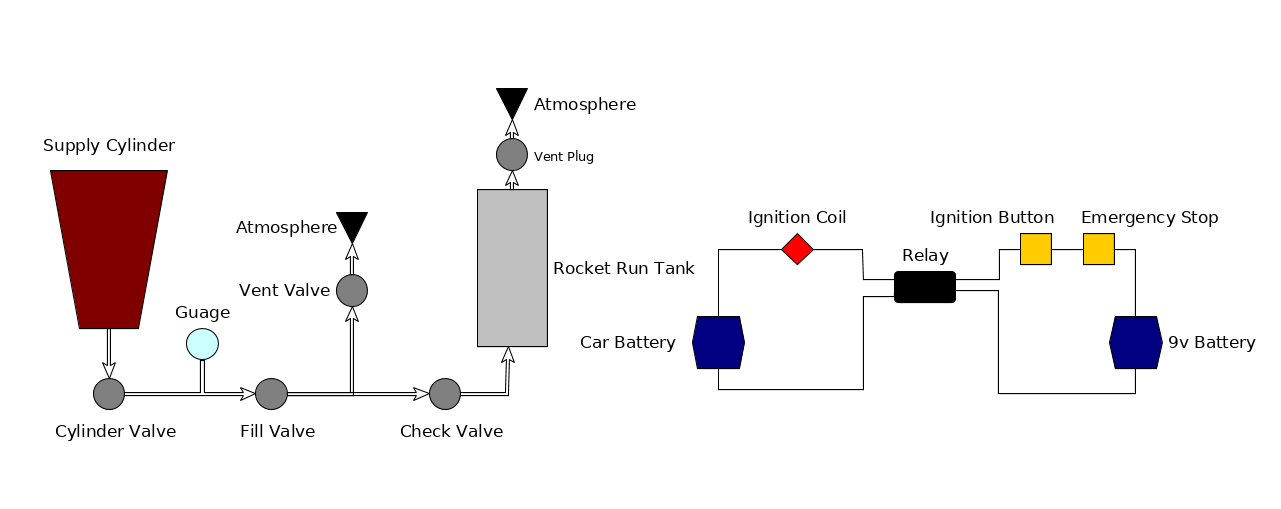
\includegraphics[width=.9\linewidth]{./images/old_system.png}
\caption{\label{fig:org18a0954}
Launch system for 2016}
\end{figure}

The fill system is composed of the supply cylinder, the 4 valves, the gauge, the
vent plug, and the rocket's run tank. In order to fill the rocket, the cylinder
valve would be opened, the supply pressure would be checked on the gauge, then
the Fill valve would be opened, while the vent valve was left closed. The check
valve allows nitrous to flow into the run tank, but not back out. The vent plug
was a small hole in the top of the run tank that allowed the air to escape while
nitrous flowed into the tank. Once the run tank was full, the fill valve would
be closed and the vent valve would be opened, allowing the lines to depressurize
before they were disconnected from the rocket. The check valve prevented the run
tank from depleting once the fill lines were removed.

All of these valves were manually controlled. Two people, wearing the proper
PPE, would turn the valves and remove the fill lines from the rocket by
hand. This was allowed by the competition rules until 2017, when the safety
restrictions were increased.

The ignition system is shown in the right side of that image. In order to light
the engine, current was passed through the ignition coils, which was made of
nichrome. Nichrome is the same material used in an electric stove's
burners. Passing sufficient current through the ignition coil sparked a fire in
the engine's combustion chamber, which launched the rocket.

The current through the ignition coil was controlled with a relay. A relay is
an electrically actuated switch. By passing a small amount of current (\textasciitilde{}100 mA) through
the \emph{coil} side of the relay (the two connections on the right side of the relay
in the above image), the two \emph{switch} contacts (the connections on the left
side) would be shorted, allowing a much larger current (\textasciitilde{}3 A) to flow through
the ignition coil. Many more relays are used in the modern version of RLCS, so
understanding their operation is important. More information can be found on
\href{https://en.wikipedia.org/wiki/Relay}{Wikipedia}.

\subsubsection{Ignition testing}
\label{sec:org7495877}

At the competition in 2016, the ignition system failed to cause the rocket to
launch. As such, much of the development effort in the fall term of 2016 was
spent on redesigning the ignition system. As a part of these efforts, an
additional ignition coil was added to the system, in parallel with the
first. This increased redundancy in the system: if the primary coil failed to
cause the rocket to launch, we could try again on the secondary
coil. Fortunately, we have never (at competition or in testing) had to fall back
to the secondary coil, but the option is there. During this competition cycle,
we also upgraded the car battery to an 11.1V Li-Po battery, which was smaller,
cheaper, and lighter.

\begin{figure}[htbp]
\centering
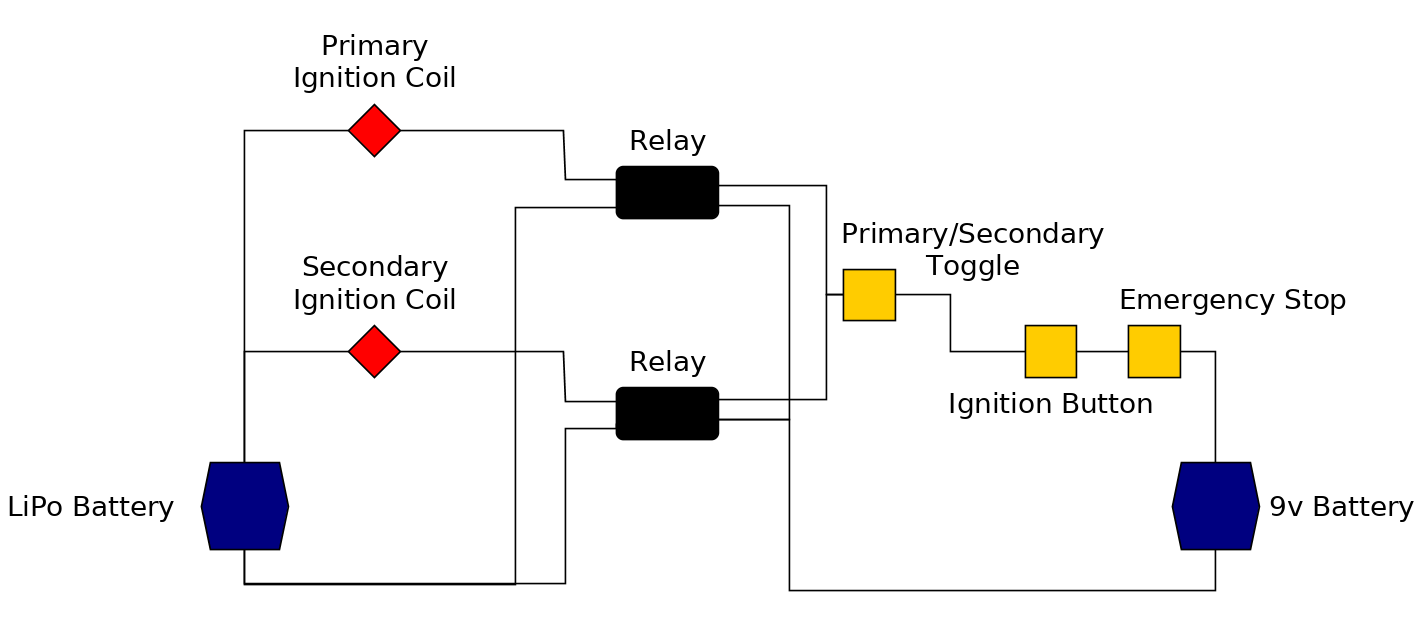
\includegraphics[width=.9\linewidth]{./images/tsig.png}
\caption{\label{fig:org3291e70}
Ignition system for IREC 2017}
\end{figure}

\subsection{RLCS V1}
\label{sec:org9541d10}

Everything changed when we got the documents for SAC 1. The rules for the new
competition stated that we had to be at least 2000 feet away from the rocket
while it filled and launched. Our current system at the time did not allow us to
fill the rocket remotely at all, and ignition could be controlled a maximum of
200 feet away. We didn't think that it was possible to get enough wire to
control all of the valves and ignition from 2000 feet (which later became 3000
feet) away, so we knew we needed to do something wireless.

\subsubsection{Why I was put in charge}
\label{sec:orgd2ffc91}

These issues were discovered early in the spring 2017 term. During that term,
most of the team (including all of the senior members) were on coop. The only
three members on stream were Jacob, Alex and myself. Alex had the most
experience with electronics, but she was busy with school and DAQ, and wouldn't
be coming to competition due to 2B labs. So the project just kinda defaulted
onto me. I was in charge of setting up a radio link that could control ignition
and two valves (the fill and vent valves). Fortunately, I didn't have to deal
with the motorization of the valves and the driving of them, David volunteered
to do that, and a lot of the assembly was done by Remy.

\subsubsection{Remote fill and TSRF}
\label{sec:org0f8a52e}

TSRF stands for "Tower Side Remote Fill". It was the box that controlled the two
electrically actuated valves that we used at IREC 2017. Electrically controlled
valves are pretty common in industry. Unfortunately, because they're industrial
components, they cost a lot. Like, \$500 each a lot. Fortunately Dan was nice
enough to sponsor us for two of them, and David bought a third. So we had
valves. The way to drive the valves was pretty simple: they had 4 wires coming
out of them, red, black, blue, and white. To open the valve, you shorted the red
wire to 12V and the black wire to ground, while leaving the other two wires
disconnected. To close the valve, you shorted the blue wire to 12V and the white
wire to ground, while leaving red and black disconnected. It's super simple to
drive these valves with a \href{https://en.wikipedia.org/wiki/Relay\#Pole\_and\_throw}{DPDT relay}, as is shown in the images below

\begin{figure}[htbp]
\centering
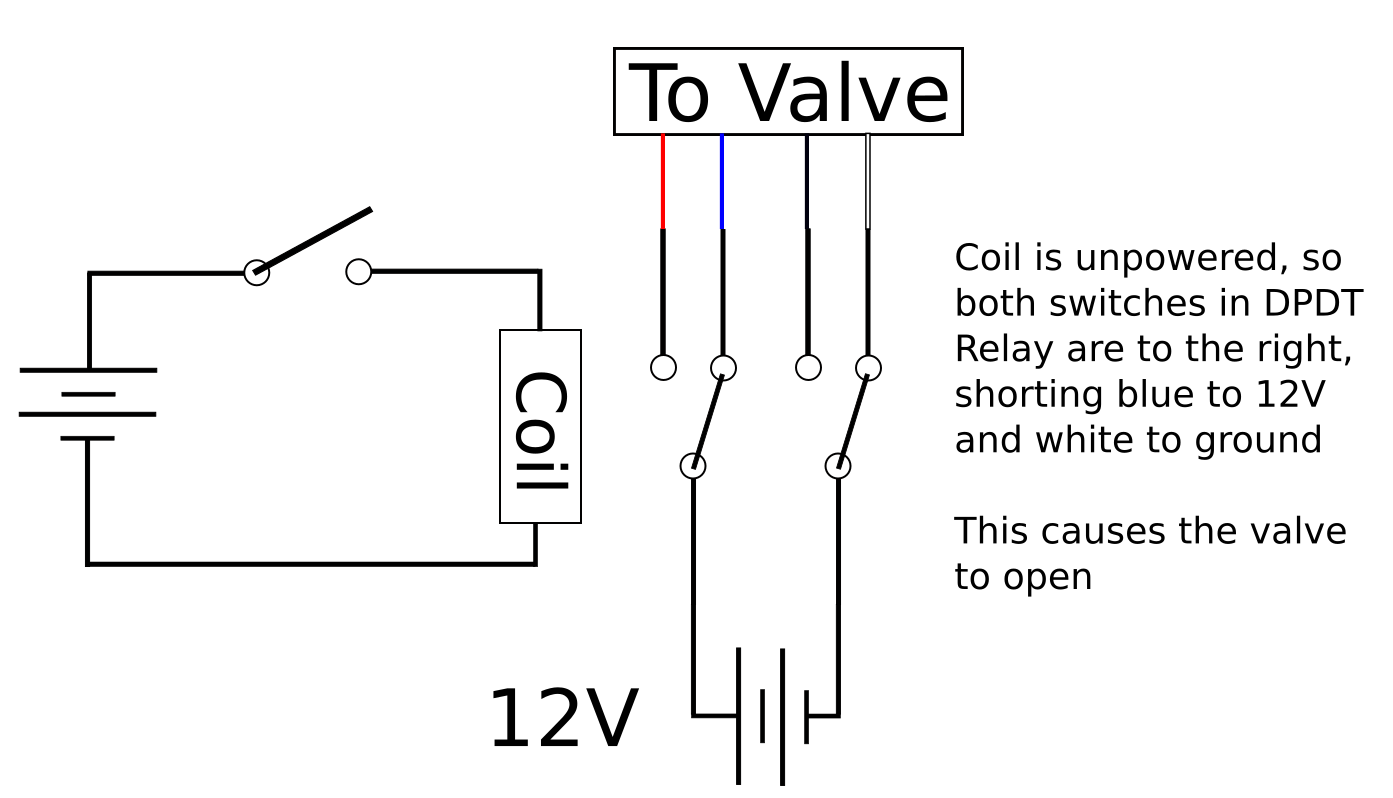
\includegraphics[width=.9\linewidth]{./images/dpdt_opening.png}
\caption{\label{fig:orga38b287}
DPDT relay opening valve}
\end{figure}

\begin{figure}[htbp]
\centering
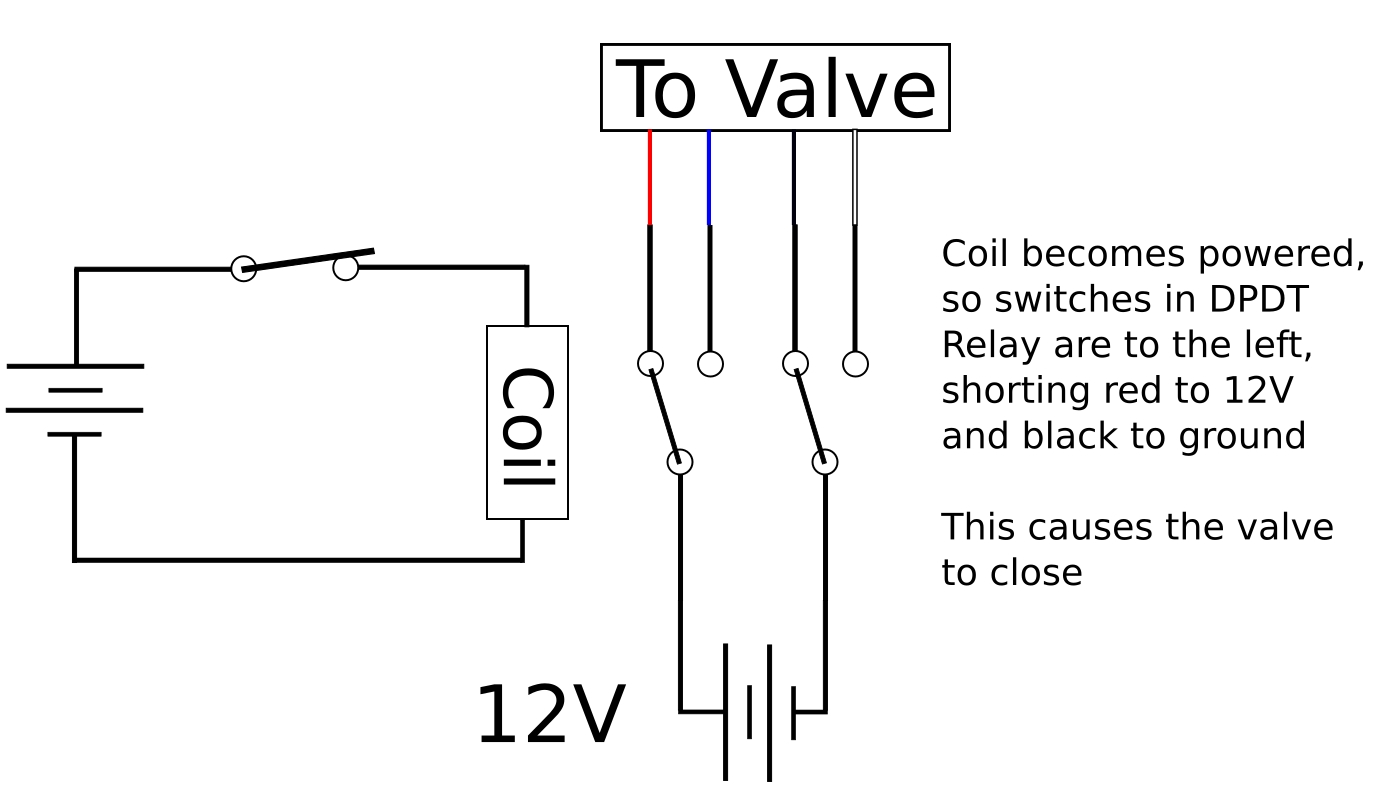
\includegraphics[width=.9\linewidth]{./images/dpdt_closing.png}
\caption{\label{fig:orgfd0a9ba}
DPDT relay closing valve}
\end{figure}

As an aside, in 2017 we didn't actually use DPDT relays to drive the valves, we
used a bunch of SPST relays because they were cheaper. If you want, you can dig
through the slack archives to find pictures and schematics for TSRF, but they
don't really fit into this document.

Because David and Remy were working separately from me on the remote fill
controls box, there was a great deal of separation between ignition, radio
communication, and remote fill control on the tower side of RLCSv1. The ignition
box used at IREC 2017 was the same circuit as we were using in ignition tests,
but put into a tiny black plastic box (life advice, if you're planning to leave
an electronic system in the New Mexico desert sun for days on end, don't put it
in a black box). That box was renamed to TSIG, "Tower Side IGnition".

\subsubsection{TSC - do as little as possible to make it work}
\label{sec:orgc3ad791}

TSC, or "Tower Side Control", was the box near the tower with a radio antenna on
it. This box controlled, via some small signal relays, the larger relays in TSIG
and TSRF. The box had an Arduino in it, which talked over UART serial to an
XBEE, which did all the radio communication. The Arduino listened for commands
from the radio, and toggled the signal relays, which toggled the bigger relays,
which opened valves or fired ignition or extended/retracted the linear actuator
(the actuator was what pulled the fill hose out of the rocket).

\subsubsection{CSRF and CSIG}
\label{sec:org3b7548b}

On the client side of the MSD were two boxes, named CSRF (Client Side Remote
Fill) and CSIG (Client Side IGnition). CSRF contains the switches for all of the
valves and the linear actuator, as well as the radio for communicating with the
tower. Each valve had two switches on the box, one to control the direction
(switching this caused the DPDT relay connected to the valve to switch), and one
to control power (switching this caused another SPST relay that was in series
with the battery to be switched. When the power switch was off, the valve did
not move). The CSIG box wasn't actually a box, but was a 2x4 with the same two
buttons mounted on it as we used in ignition testing. It had a cable on it that
ran into CSRF, whose Arduino read the state of all the buttons and updated the
tower.

The reason that the buttons for toggling ignition and for toggling the valves
was entirely FBE based. Yash had a dream that we accidentally fired ignition
while trying to toggle a valve, and because of that dream we kept the controls
in separate boxes in order to reduce the chance of mispressing a switch. I kid
you not, we made engineering decisions about this system based on a dream
someone had. This story isn't \emph{relevant} in any way, I just thought it was fun.

\subsubsection{The code}
\label{sec:orgdacf1c2}

All the code from RLCSv1 is backed up on GitHub,
\url{https://github.com/waterloo-rocketry/rlcsv1}. There's about 600 lines of code
between the tower side box (TSC) and the client side box (CSRF). There's also
two plain text files named client/tower\_pseudocode.txt, which explain pretty well
what the code is doing. RLCSv2 has a much larger and more complicated code base,
so reading this code is probably a good introduction, since the v2 code grew out
of this.

The loop for the client side mostly looks like this (at least as far as ignition
and valves are concerned):
\begin{itemize}
\item Read all of the buttons and switches
\item If it's been longer than 1 second, ask the tower what state the valves and
igniters are in:
\begin{itemize}
\item If that disagrees with what the buttons say, tell the tower to change to be
what the buttons are
\end{itemize}
\item If the tower is asking us to acknowledge a state change (opening a valve or
firing an igniter):
\begin{itemize}
\item If it's changing to the state we want it to, respond with an ACK
\item Else, respond with a NACK.
\end{itemize}
\item Update the information on the LCD (more on that later)
\end{itemize}

The loop for the tower is mostly this:
\begin{itemize}
\item If there are any bytes from the radio:
\begin{itemize}
\item If the client is asking for our state, send it
\item If the client is telling us to change our state, ask for an ACK
\item If the client has given us an ACK, change state
\end{itemize}
\item If it's been more than 10 seconds since we've heard anything from the client,
immediately close the fill valve and turn off ignition (go to safe state)
\end{itemize}
\subsection{The move to V2}
\label{sec:org64bece1}

After IREC 2017, there were a lot of things I wanted to change about RLCS. I
even wrote a whole document outlining the reasons I wanted to upgrade it, how I
thought it best to go about doing so, and how much I thought the whole thing
would cost. I'll try to explain the reasons for the switch here as well, but if
you want an even more complete backstory of RLCS, that project proposal can be
found on GitHub at
\url{https://github.com/waterloo-rocketry/rlcs/blob/master/dev\_logs/official\_project\_proposal.pdf}.

\subsubsection{Things to Fix}
\label{sec:org0dd499f}

There were a lot of things that I hated about RLCSv1:
\begin{itemize}
\item I wanted to move everything into 2 boxes, one at the tower and one at the
client, for robustness reasons (cables kept breaking on v1).
\item I wanted to have limit switches on the valves so that we knew whether or not
they had turned properly. In v1, we relied entirely on visual feedback to know
when the valves had moved (David stood 3000 feet away from the rocket with
binoculars to try to see if a valve on the ground had turned. No it did not
work well).
\item I wanted the system to be more extensible, and easier to add more valves
to. There was some talk around this time of building a super-pressurized
rocket, which would have required 2 more valves. These 2 valves would have
been a pain to add to RLCSv1, since the whole thing was hand soldered on
veroboard.
\item I wanted better radio contact (if you stood near TSC back in the v1 days, the
boxes lost the ability to communicate. Which was scary). I wasn't sure at the
time how to do this, and there are still improvements that could be made
towards this end, but we suffered no such problems in 2018, so it's no longer
a priority for me. We never wound up changing the radios or antennas, we just
mounted the tower side antenna 25 feet up the tower. Radio antennas like being
up high to avoid fading.
\item I wanted to log everything that happened in the system onto an SD card. This
we did do, but I never wound up looking at the data. It was mostly for failure
analysis anyways.
\end{itemize}

\subsubsection{Extensibility (PCBs)}
\label{sec:org34b0ba2}

The first problem we solved was the extensibility problem. All of the actuators
(ignition coils, electric valves, and linear actuator) can all be controlled by
the circuit shown in figure \ref{fig:orgc4748df}. For the ignition coils, if you want
to fire them, you just do as is shown in figure \ref{fig:org5d1220c}. When the coil
is energized, the switches move over and short the ignition coil across the 12
volt battery. The linear actuator is slightly more complicated, but can still be
driven by the same circuit.

\begin{figure}[htbp]
\centering
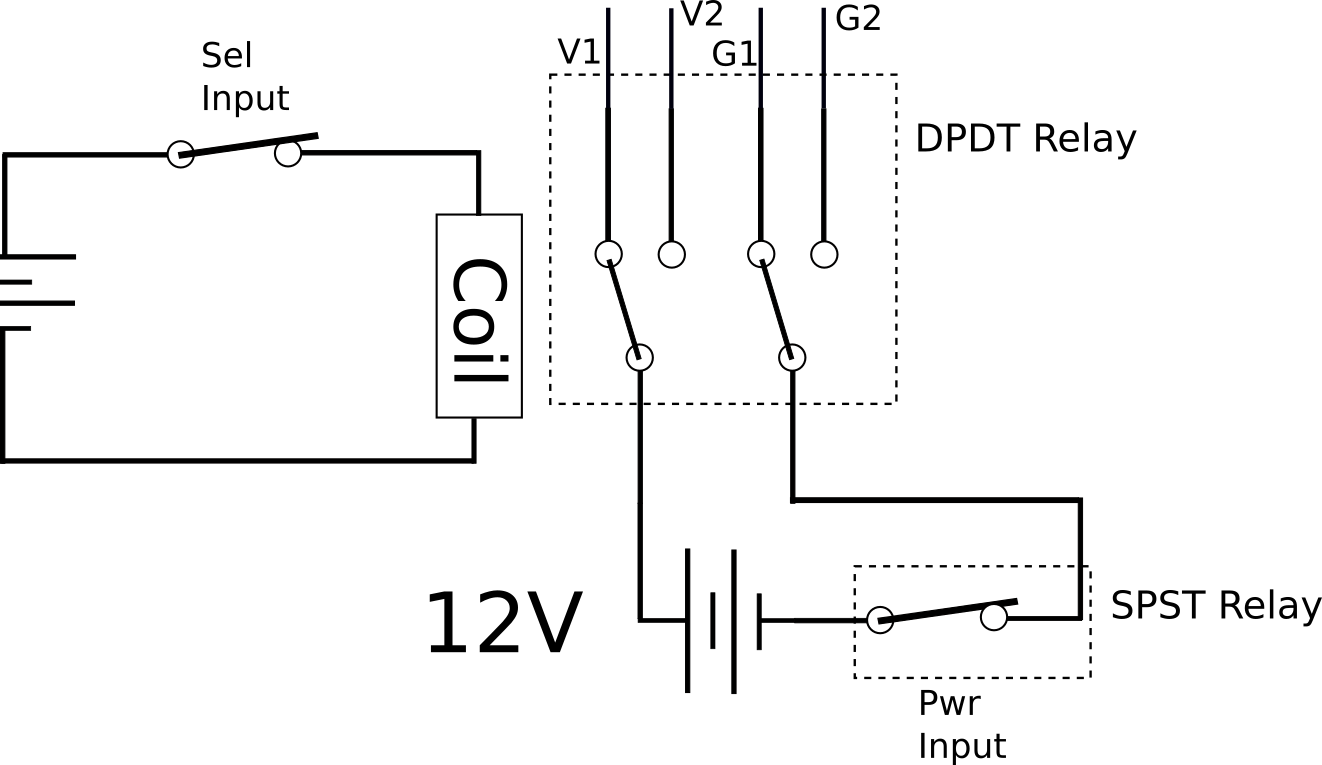
\includegraphics[width=.9\linewidth]{./images/pcb_general.png}
\caption{\label{fig:orgc4748df}
Circuit capable of driving all the actuators}
\end{figure}

\begin{figure}[htbp]
\centering
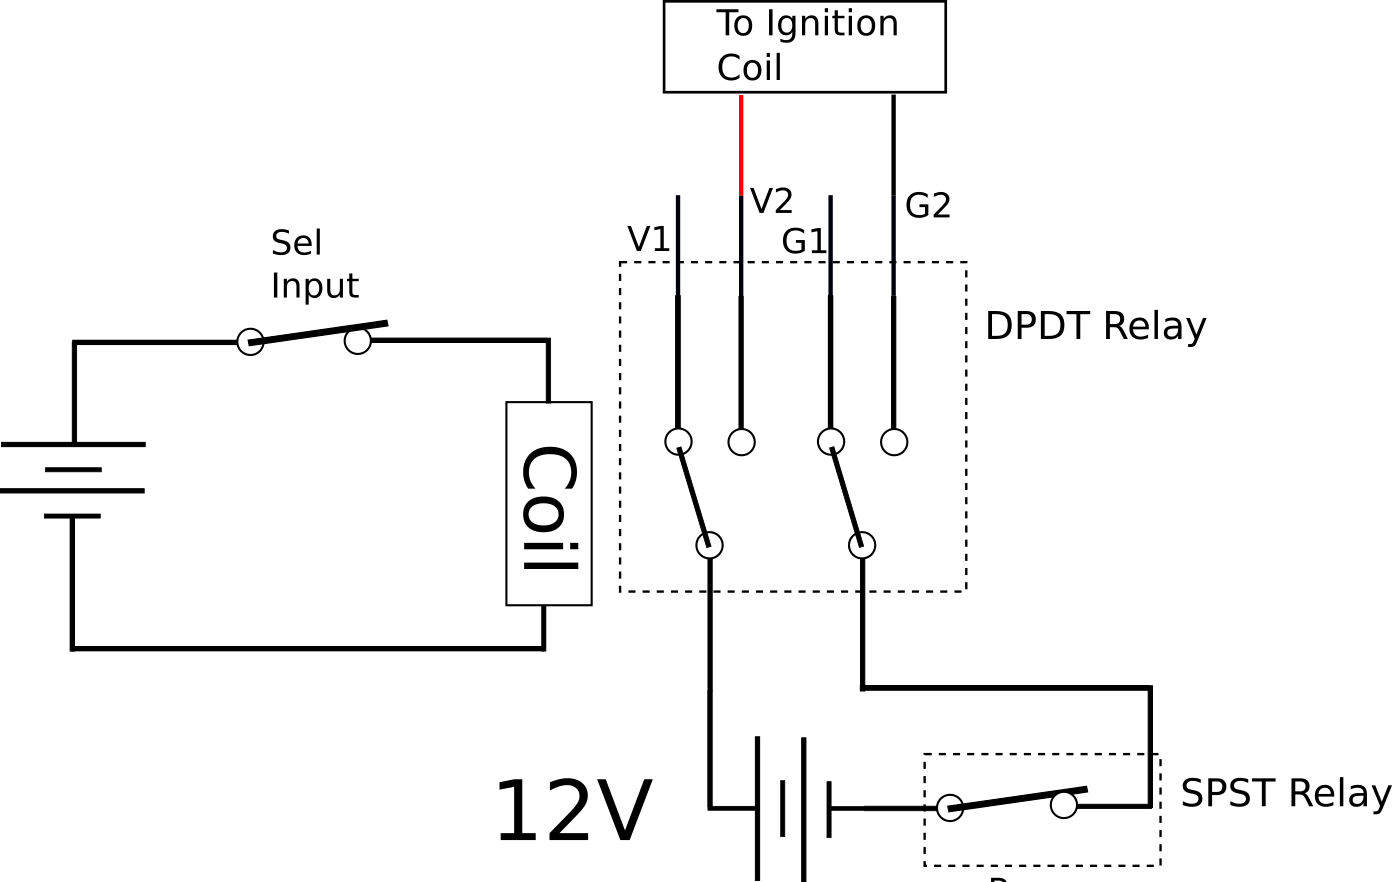
\includegraphics[width=.9\linewidth]{./images/pcb_ignition.png}
\caption{\label{fig:org5d1220c}
Wiring that circuit for ignition}
\end{figure}

\begin{figure}[htbp]
\centering
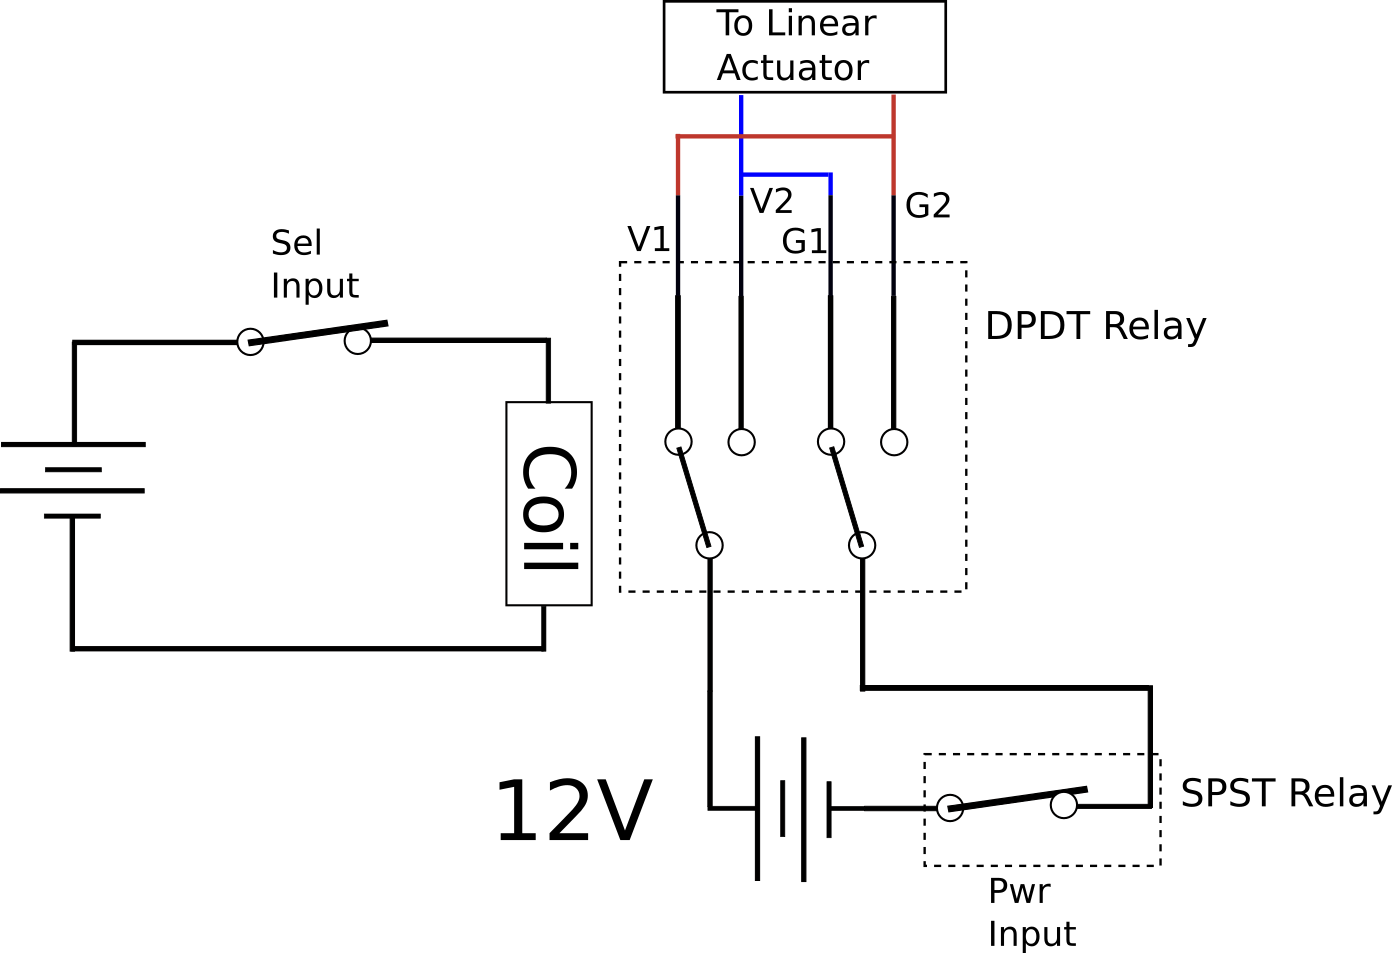
\includegraphics[width=.9\linewidth]{./images/pcb_linear_act.png}
\caption{\label{fig:orgfdcfd88}
Wiring that circuit for linear actuator}
\end{figure}

The linear actuator has two wires coming out of it, one with blue insulation and
one with brown. If you apply 12V to the blue wire and short the brown to
negative, the linear actuator will extend. If you swap them (brown -> 12V, blue
-> GND), the linear actuator will retract. If you wire the linear actuator to
the DPDT relay in the way shown in figure \ref{fig:orgfdcfd88}, then you can
control its direction. energizing the DPDT coil changes the direction of the
linear actuator, and energizing the SPST coil applies power to it.

So we made PCBs with this circuit on them. Each one of these PCBs could drive a
single actuator (well, you could conceivably drive both ignition circuits from
one PCB. We don't because reasons. See the explanation in section
\ref{sec:linear_act_lsw}). Each PCB also has some additional features for
actuator feedback, more on that in the subsection about DAQ. They also all got
fuses on them, for no real reason. The fuses are in series with the power in
blocks, so if the fuse blows no more current goes out to the actuator. In theory
this should prevent things from catching on fire, in practice we've managed to
burn some stuff without the fuses blowing (see appendix on linear actuator limit
switches).

There are 17 wires coming off of each PCB (sorry). 6 are for the actuator, 4
being for power and 2 being for limit switches (more on the limit switches in
the DAQ section). You've already seen how the 4 power ones are laid out. They're
labeled V1, G1, V2 and G2. When the DPDT relay is not powered, V1 is shorted to
12V and G1 is shorted to ground, and the other two connections are open. When
the relay is powered, it's the opposite (V2->12V, G2->GND, V1,G1 open
circuit). The other two large wire inputs are for power, these run directly to a
lipo battery.

There are 9 small wires going into the PCB. 4 of these (I1, I2, L1, L2) are for
actuator feedback, there'll be more about them in the DAQ section. 3 are for
power (5V, 12V and GND). The power for these is provided from the same battery
powering the Arduino. The 5V rail is used for the current amplifiers (more on
them later), and the 12V input is used for the coils of the relays. The reason
that this 12V input is not shorted to the actuator power input 12V is for
extensibility: When I was designing these boards I was not sure that we would
always be using them to drive 12V DC actuators. In theory (do not try this
unless you know what you are doing), you could use these PCBs to drive 120v AC
valves by applying 120v AC to the actuator power inputs, without affecting the
relays. We have never tried this.

The remaining 2 inputs are the SEL and PWR inputs. These drive the relay coils
(they go through a transistor in order to allow the 5V signal coming from the
Arduino to control a 12V signal to power the relays, but that's neither here nor
there). When the SEL input is pulled to 5V, the DPDT relay switches. When the
PWR input is pulled to 5V, the SPST relay switches. In order for these relays to
switch, the 12V and GND small power connections must be present.

\subsubsection{Tower side box}
\label{sec:orgcb56c84}

Once we had the PCBs, all we needed was a box to put them in. This is the big
silver box you can find under the electrical bench. In V1 we had three tower
side boxes (one for each of ignition (TSIG), remote fill (TSRF) and control
(TSC)). All three of these boxes merged into what we now just call the Tower
Side Box. A rough schematic of how the electrical connections of the tower side
box is below.

\begin{figure}[htbp]
\centering
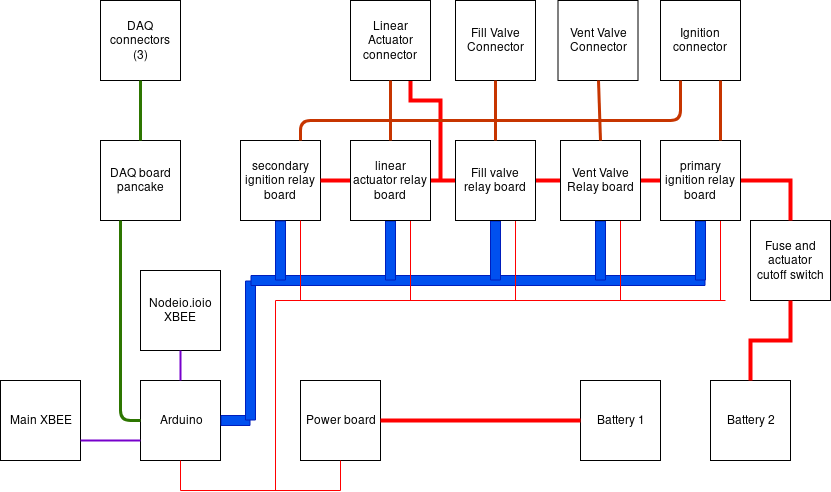
\includegraphics[width=.9\linewidth]{./images/tsb_full.png}
\caption{\label{fig:orga8d53f0}
All the connections inside the tower side box}
\end{figure}

The reason for the split between batteries is historical largely: In V1 there
were separate batteries in TSIG and TSRF, with the intention of not draining the
battery driving the Arduino when a valve turns. Hence, we have one battery for
powering the radio and Arduino, and another for powering the valves and other
actuators. There is some logic to this, when you start drawing a lot of power
from a battery, its voltage drops. If the voltage to the Arduino drops
momentarily, the Arduino could reset. Which would be \emph{safe} (at startup, it
closes the valves), but inconvenient. At one point, we thought that there would
be two batteries in parallel for driving the actuators, but they don't actually
burn that much power so there's no real point. Also, putting LiPos in parallel
can be dangerous if their charge levels are different. So don't do it.

Note the switch in series with the actuator battery. Usually when you can't
figure out why the actuators aren't working ("It seems like the relays are
clicking, but the valve just won't turn"), it's because this switch is turned
off. Make sure to turn it on before any tests.

There's nothing really fancy about the power converter PCB, although it looks
like there is. It takes in 12V and spits out 5 (and also 3.3 and 15, but we
don't use those). It also has an SD card and a seven segment display on it. More
on how those work in the Code Changes section.

There are a lot of wires in this box. Each of the green PCBs has 7-10 wires
coming out of it, and there are 5 of those PCBs. Just remember that everything
is modular, so it's really just the same circuit repeated 5 times. If that helps
at all.

Fun fact about the box BTW: We were originally trying to get pelican to sponsor
us a really good plastic hardcase, but they never emailed us back, so we put
everything in the shiny briefcase that Jacob got from his coop job at
teledyne. In order to make the bottom heavier (so that the box wouldn't tip
over), Alex epoxied a bunch of 2x4's into the bottom of the box. Which is why
it's so goddamn heavy.

\subsubsection{Client Side box}
\label{sec:org3be7efb}

Similar to the tower side box, the client side boxes all merged into
one. Ignition and remote fill controls are both in the same box this time, and
the LCD was made larger (V1 had a 16x2 character display, V2 has a 24x4 I
think. Maybe 40x4, I'm not sure). The LCD also received a contrast adjust
potentiometer. It may seem like this thing doesn't do anything, but it's very
important. When LCD's get hot, their crystals deform and you lose the ability to
read them. The contrast knob adjusts for that. V1 didn't have one of these,
which worked fine. Until we brought it into a desert. Fun fact, Miranda launched
Vidar III Mk II without being able to read the goddamn LCD on the launch box.

It also moved into a much better box. Instead of a crappy plastic box we
inherited from Yash's FYDP that they bought at Sayal plugged into a 2x4, it's
now in a pelican hardcase. I bought this hardcase from a guy from Kijijii for
\$25. The team never paid me back. Because of the laser cut wood panel on there
(designed by Kylie), this box is the most professional looking box that our team
owns. We bring it out at Open Houses sometimes.

A rough electrical schematic of the box is below.

\begin{figure}[htbp]
\centering
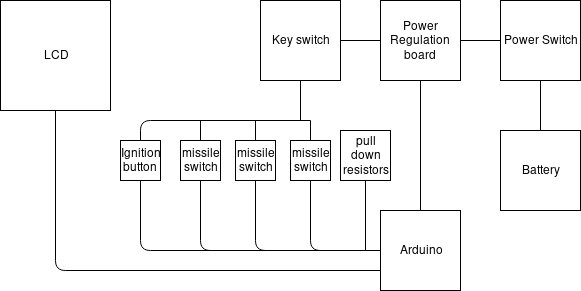
\includegraphics[width=.9\linewidth]{./images/csb_full.png}
\caption{\label{fig:org299422c}
All the connections inside the client side box}
\end{figure}

Note the Safety key switch: When this key is off, all of the actuator switches
lose power (which has the cool effect of making their LEDs turn off). Note that
the Arduino has no way of distinguishing whether the safety key switch is off or
whether all of the actuator switches are now turned off. Because of this, when
you turn the safety key, all of the valves will close. This is on purpose. But
be aware of it.

The power converter PCB is the same as the one in the tower side box. Yay
reuse. It has the same SD card and 7-segment display as the tower side box. The
7-segment display shows the state that the box is currently reading from the
switches. I don't have it memorized what each state works out to in numbers, but
this is good for debugging. If you flip a switch, and the seven segment display
value does not change, that means that the Arduino is not reading the switches
properly. It could be that the pull-down resistor came undone, or it could be
that the switch is dead, but at least you know.

The only other change is the removal of the emergency stop switch from the
ignition buttons. The competition is kinda scared of us accidentally firing our
rocket, so their rules state that you need two actions to fire ignition. In V1,
those actions were "disengage e-stop, push fire". In V2, we have the same fire
switch, but two arming missile switches (one labeled primary, one labeled
secondary). 

\subsubsection{Code changes}
\label{sec:org47e6b6c}

The code was entirely rewritten when moving from V1 to V2. And the codesize
exploded. We went from about 1000 lines of code in 2 files to about 3000 lines
of code spread across 28 files (I thought doing this would make the codebase
simpler. It did not, in fact, make it simpler). It's mostly separated out into
functionality, ie everything to do with logging to the SD card is in
sd\_handler.cpp and sd\_handler.h. Some of the files are only used by one of the
two Arduino's (the tower side or the client side), but some are shared. All of
this is discussed in the Code section of the "System as it currently exists"
section.

\subsubsection{DAQ}
\label{sec:orgdfd014e}

During static fires and cold flow tests in Waterloo, we use the DAQ system to
monitor how much nitrous has been loaded into the rocket, and what pressure that
nitrous is at. We need access to this same information at competition (we need
to know when the rocket is done filling so we can launch it), but we don't have
the DAQ system at competition. Instead we plug those sensors into RLCS.

We had this system in V1 as well. We would read two pressure transducers and one
load cell using an Arduino's onboard ADC. The problem came when we needed to use
strain gauge based pressure sensors instead of the preamped piezo based ones we
were using in 2017 (talk to the DAQ people about what these words
mean). Suddenly we needed instrumentation amplifiers in RLCS. So we added an
amplifier board that the two pressure transducers plug in to. There are
connectors for these sensors on the tower side box.

The data from these sensors is sent back from the tower side box to the client
side box over the same radio link as the actuator states. The code for sending
back the DAQ data is almost identical to the code used for the actuator state
stuff, so it isn't really explained in this document in great detail.

\subsubsection{Flight instr}
\label{sec:org429993c}

You can probably skip this section, since flight instr has been replaced by
busproj.

In 2018, we went from VIDAR III to UXO. UXO was far more complicated in many
ways than VIDAR, especially in terms of electronics. UXO had two valves onboard,
one to vent nitrous from the run tank and the other to allow nitrous to flow
through the injector. It also had two pressure transducers onboard, in order to
monitor the pressure of the nitrous as well as the pressure inside the
combustion chamber. We needed electronics in order to control these valves and
sensors, and we needed a way of communicating with these electronics at launch
time.

Enter Flight Instrumentation. It was a project to put electronics into the
rocket to control valves. There were two boards (named after the Gilmore Girls),
one above the oxidizer tank and the other in the injector section. Both of these
boards had radios onboard, and those radios communicated with another radio
inside of the RLCS tower side box. This radio network was completely separate
from the radios communicating from tower side box to client side box. Both
boards also had SD cards on them, so that the data from the pressure transducers
(as well as some onboard accelerometers) could be logged for later reading.

Flight Instrumentation never \emph{quite} worked perfectly. Due to project timelines,
the system was never tested fully and the data logging happened at a slow rate,
so the data wasn't very useful. It worked to launch the rocket though, so the
first objective was a success. The project has been superseded by busproj, so
flight instr will only have been used for one year. If you want to dig into the
code that the tower side box used to communicate with the two systems in the
rocket, you can look through \textbf{nodeio.ioio.cpp/.h}. The network was named that
(nodeio.ioio) because I thought it was funny.

\section{The system as it currently exists}
\label{sec:orgfaa273c}

\subsection{Drawing}
\label{sec:orgc78e79c}

TODO, draw the entire system, label each component, and describe what each
component does, briefly.

\subsection{Setup instructions}
\label{sec:org07f2591}

\subsubsection{Required items}
\label{sec:org543765a}
\begin{enumerate}
\item Tower side box (big, briefcasy, and silver)
\item Tower side radio box (small white 3d printed box with an antenna sticking
out)
\item Cable that goes from 1. to 2. It's a CAT5 cable, and it's got two RJ-45
connectors on it, but note that it is \textbf{NOT} wired like a normal Ethernet
cable. Don't just plug any cable in here, something might blow up.
\item Both electric ball valves. They should have a long thick grey cable coming
out of them.
\item Ignition cable. Same thick grey cable, but it terminates in 2 quick connect
cables, one should have a P sharpied on it and the other should have an S
(those stand for primary and Secondary).
\item The linear actuator cable, which should go into a linear actuator.
\item Load cell and 2 pressure sensors, with cables coming out of them that match
the DAQ connectors on the tower side box.
\item Client side box (Yellow with a rocketry sticker on the top)
\item Client side radio box (same 3d printed box, but this one has a cat-5 cable
coming out of it, which is duct taped in.
\item 3 lipo batteries (check that they're charged. 1 goes in client side box, 2 go
in tower side box).
\end{enumerate}

\subsubsection{Setup the tower side box}
\label{sec:org50cf548}
You'll need two LiPo batteries for this part. One plugs into the deans connector
leading to the power PCB. This will turn on the Arduino, radio, and power all of
the relays. The other plugs into the deans connector leading to the relay
boards. Note that there is a fuse and a switch in series with this battery
before they arrive at the PCBs. Until you're ready to test, leave this switch
off.

Plug in the radio to the RJ-45 connector on the side of the box. The LEDs on the
radio should illuminate when you do this, if they don't: check all of the
connections leading from the battery powering the Arduino to the radio, there
should be 6 of them (batt->power PCB, power PCB->red wire, red wire->female
RJ-45, female RJ-45->cat 5 cable, cat 5 cable->radio box, radio box->radio PCB)

Plug in the actuators to the connectors at the back of the tower side box. These
connectors are keyed, they only plug in one way. The connectors on the box
should be labeled (IGN for ignition, FILL for remote fill valve, VENT and
DISCONNECT for remote vent valve and linear actuator connections).

Flip the actuator power switches. This should cause the two valves to close, if
they are open. Check that the ignition connectors are not powered (check with
multimeter). If they are, it's possible that you plugged a cable into the wrong
spot.

Plug in the DAQ connectors for the load cell and 2 pressure transducers. This
step is not necessary during static fires and cold flow tests, RLCS is only used
with these sensors at competition.

\subsubsection{Setup the client side box}
\label{sec:orgea0a775}

Remove the wooden plate from the client side box, so that you can access the
power connector. Plug this into the battery, and put the plate back into the
client side box. Flip the large black switch to power the system. The LCD should
light up and display some values. The red Connection Bad LED should light up,
since the radio is not plugged in. Turning the arm switch should cause the
actuator missile switches to illuminate.

Plug in the radio box. The blue Connection Good LED should illuminate after a
few seconds. If it does not, then you need to debug the radio connection. Some
ideas of how to do that are in the appendix, but it's impossible to document all
of the ways that the radio connection could be failing. My advice in this
instance is to try to isolate the failing component as best as you can. To do
this, find all the points at which the system is working properly (ie, the
Arduino is sending the right data, it's just not being received by the
radio). The failing component must be between the points where the system is
working. It will usually be a problem with a connector somewhere, but it could
be a broken radio or radio communication PCB.

\subsubsection{Test that everything is working correctly}
\label{sec:org5fd4be5}
Make sure that when you flip a switch on the client side box, the associated
actuator on the tower side box moves. Check this with both valves and the linear
actuator. Use a multimeter to ensure that when you fire ignition (arppming one of
the ignition circuits (but not both. You can't fire both ignition circuits at
once, the code treats that as an error) and pressing the red fire button), one
of the ignition circuits goes to 12V. Test the other ignition circuit as well.

Check that the DAQ sensors are working as well (if you're using them). Ensure
that the pressure sensors are reading close to atmospheric, and that when you
apply force to the load cell, the reading on the client side box changes.

If any of this doesn't work, you'll need to debug it and get it working. I
highly recommend going through this process at least a week before any actual
rocket test, because you want to know that this works before we're all ready to
go. If parts are broken, you'll need at least a few days to order them in from
digikey. Plan for this, debug early.

\subsection{The code}
\label{sec:org66fd929}
\subsubsection{The common code}
\label{sec:org9fbc1f9}
The stuff that's used in both Arduino's
\begin{enumerate}
\item The SD card library:
\label{sec:orgd37c3df}
Both the tower side and client side boxes have SD cards in them to log data. As
such, the \textbf{sd\_handler.h/.cpp} library is run on both. This code depends on the
Arduino \textbf{SD} library, and provides some helper functions that log data to the SD
card. For example, \textbf{rlcslog(string)} logs the string that is passed to it.

This library supports some amount of buffering before sending the logs to the SD
card for performance reasons (it's equally fast to save 1 byte to an SD card as
it is to save 512 bytes, so you might as well wait until you have 512 before
saving anything). This means that just calling \textbf{rlcslog} won't save anything to
the SD card, you also have to call the \textbf{flush()} function in the library to make
it save what it has onto the card. You can tell whether or not the library has
any data buffered with the \textbf{sd\_buffer\_dirty()} function, which returns true if
there's any data not yet saved. The client side box shows this to the user on
the LCD, there's a line that says \textbf{SD: OK} if all the data has been saved, \textbf{SD:
DI} if the data has not all been saved, and \textbf{SD: NO} if it couldn't initialize
the SD card.

This library has an init function (\textbf{sd\_init()}) that needs to be called in the
setup function of both Arduinos.

\item The Seven Segment display library
\label{sec:org5949596}
Similar to the SD card, both boxes have a seven segment display, so this library
drives both of those. It's possible that the two Arduino's will use different
pins in order to drive the seven segment display. To accommodate this, both boxes
have files called \textbf{tower\_pin\_defines.h} or \textbf{client\_pin\_defines.h} which indicate
which pins are to be used by this library.

The library has a function called \textbf{refresh\_SevSeg()} that has to be called every
loop, which re-flashes the numbers on the seven segment display. To change the
number shown, the function \textbf{setNewNum\_SevSeg(number)} has to be called. The
tower side box uses this library to show what state it thinks it should be in,
the client side box also uses it to show what state it thinks the tower should
be in, based on the switches. The only one of these that really matters is the
state \textbf{04}, which is the "safe state" of the tower box. If the tower side box
hasn't received anything from the client side box in 10 seconds, it flips to
state \textbf{04}. This is the quickest way to see if the two boxes are communicating
properly (ie the radios are working). If the seven segment display on the client
side box shows a number that is not \textbf{04}, but the tower side box shows \textbf{04},
that means they can't communicate, and you need to debug the problem.

\item The shared types library
\label{sec:org362d36f}
There are two types (classes if you're a C++ guy) that are used in both the
client side and tower side boxes. One is the DAQ type, which will be talked more
about in the DAQ section, and the other is the \textbf{actuator\_state\_t}. The
\textbf{actuator\_state\_t} holds a bit for every actuator that RLCS knows about (those
are the remote fill and vent valve, the linear actuator, and the two ignition
circuits. There's also bits for the run tank valve and injector valve, which are
discussed in the Flight Instr section). There are also functions for serializing
this struct into and out of a character (the character isn't an 8 bit character,
it's a 6 bit base64 character, but that's neither here nor there).

The advantage of sharing these serialization functions (serialization as in you
take the \textbf{actuator\_state\_t} representing the state that the client thinks the
tower should be in, you use the serialization function to turn it into a single
character, then send that character over the radio, and the tower deserializes
it and knows what state it should be in) is testability. A really annoying bug
would be if the client box and the tower box disagreed on what this character
deserialized into. Then the client box could be sending a message that it
thought meant "Fire ignition", but the tower thought it was "open the fill
valve". This would be bad. Hence, they're in the same file.

\item The radio\_comms library (\textbf{radio\_comms.h/.cpp})
\label{sec:org2829f55}
This library handles all the incoming and outgoing data through the
radios. Some of the functions in this library are only used by the client, or by
the tower, and thus have that name prepended to the function name (ie
\textbf{client\_request\_state}). These functions make more sense by looking at the radio
flow diagram of a state update shown in figure :

\begin{center}
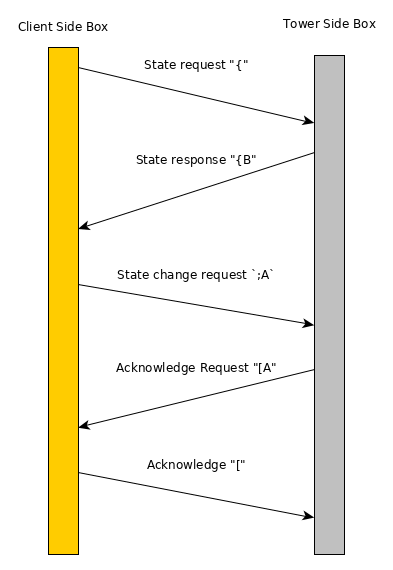
\includegraphics[width=.9\linewidth]{./images/radio_state_change.png}
\end{center}


The client asks the tower what state it's in (\textbf{client\_request\_state}). The tower
answers (\textbf{tower\_send\_state}). If the client thinks the tower should be in
another state, it tells the tower to change (\textbf{client\_push\_state}). The tower,
upon receiving a new state, asks the client if it's sure this is the state it
means (\textbf{tower\_request\_ack}). This request ack includes the state that the tower
would be switching into. If the client agrees that this is the right state, it
sends an ack (acknowledge, with \textbf{client\_ack}). If it disagrees, it sends a nack
(not ack, with \textbf{client\_nack}).

When we were first testing RLCS, the system would hang every few minutes. What
was happening was that the client was asking the tower what state it was in, and
then waiting forever for a response. If the tower didn't respond (it didn't hear
that packet or something), nothing would happen. Obviously, this was bad. Now,
the boxes repeat their last transmission forever until they hear a response. The
client will ask the tower for it's state every 100ms or so until it gets an
answer, and the client will push a new state similarly frequently until it
receives an ack request from the tower. This is why the nack command exists: If
the tower requests an ack, but the client doesn't give it, it will keep asking
forever. If the client sends a nack, the tower stops repeating its request, but
doesn't update its current state.
\end{enumerate}


\subsubsection{Tower side code}
\label{sec:orgc57cb16}

All is found in src/tower\_arduino\_ide/

\begin{enumerate}
\item Tower main loop
\label{sec:orgceb1bcd}
The main loop is found in \textbf{tower\_arduino\_ide.ino}. Following arduino standard
practice, this file contains the \textbf{setup} and \textbf{loop} functions. The setup
function initializes all of the libraries that the tower uses (the output
library, which controls the pins, the radio library for communications, the
nodeio library (See flight instr section if you really wanna know about this),
the seven segment display library and the SD card library). In the loop
function, the tower checks for any input from the client, and if it received
anything, it pushes it into its parser (called tower\_fsm). In this loop, it also
checks the time, and if it's been more than 10 seconds since it received
anything from the client, it goes into safe state, and closes all of the
valves. In this loop it also deals with the seven segment display library and
flushes data to the SD card if it's been more than a few seconds.

\item Tower FSM/radio bytes parser
\label{sec:orga86f2a7}
The FSM here stands for finite state machine, and it's that because the radio
bytes parser is a finite state machine (it's a type of parser, google it for
more information). The problem that this parser is trying to solve is that all
of the commands that can be sent over the radio take more than one byte, and
there's no guarantee that they'll be received at the same time. Take the "goto
state A" command, which over the radio looks like \textbf{;A}. The parser will receive
the \textbf{;} byte first, and go to the state called "REC\_STATE". When it's in
"REC\_STATE" (short for "receive state"), and it gets a byte from the radio, it
knows that this byte is the state that the client wants it to go to, no matter
how much time has passed since the first byte came in. This also solves the
problem of not all of the command coming through. If the tower only receives
\textbf{;}, because the \textbf{A} was dropped, it won't do anything, but it will not hang. If
the next byte it receives isn't a valid state (say it's the command for the
client requesting the tower's state, \textbf{\{}), it will know to get out of the
"REC\_STATE" state and send the client its current state. Ok I realize now that
I'm using the word "state" way too friggin often, and I apologize. Did that make
any kind of sense?


\item \textbf{tower\_globals.h/.c}, the worst named files
\label{sec:orgda69674}
These two files contain what I think of as the "global" functions and
variables. global variables makes sense, but global functions don't
really. These files mostly became a "miscellaneous" category, so it might be
best to think of them in that way. The most important of these is the
\textbf{apply\_state()} function. This is the function that takes the state
\end{enumerate}

\section{Other Stuff/Appendices}
\label{sec:org58ad61e}

\subsection{Linear Actuator limit switches}
\label{sec:org47aef76}
\label{sec:linear_act_lsw}

Aright, we have to talk about the linear actuator. Specifically, its limit
switches. An actuator will almost always have limit switches on it. The
whole point of these switches is to cut off power when the actuator reaches
the end of its stroke. For example, take the linear actuator: if the
extendy bit gets to the end of its extension, it'll hit a hard stop. If you
keep applying power once it hits this hard stop, the motor will stall, the
brushes will short through the windings (not a power engineer, don't quote
me), and it will draw several amps. This will set fire to whatever wires
are feeding power to the linear actuator. This is very bad, which is why
it's a good thing that limit switches exist.

Unfortunately, the limit switches on our linear actuator don't
work. Inside the actuator, there's a soft plastic tab that's about an inch
or so long. When the actuator reaches end of stroke, this tab hits the
limit switch. And then, because of conservation of momentum, the arm keeps
moving a little bit. Unfortunately, it keeps moving for about an inch, at
which point the tab is past the limit switch, and the power is turned back
on. So it hits end of stroke with the limit switch not hit. And things
catch on fire (we've destroyed two actuator PCBs because of this).

The solution we're running with is as follows: We turn on the linear
actuator for a very brief amount of time (100ms), then turn it off, and
repeat enough times for it to go through its full stroke. The goal is to
stop the actuator from picking up enough speed to go past its limit
switch. We don't care how long it takes for the actuator to move (it's just
pulling a pin, it can take 30 seconds for all we care), and this method has
been sufficient to keep it moving slow enough that when it hits the limit
switch, it doesn't have enough momentum to keep going past there.

All this logic for keeping track of when power should be applied vs not
applied is contained in linac.\{c,h\}.

\subsection{Ignition - why two PCBs and not one}
\label{sec:org7107fc7}

We have two ignition coils in the rocket, because we're paranoid. In 2016,
the team failed to launch three times because of ignition
problems. So we're a little touchy about ignition problems. In the 2017
competition cycle, we completely revamped the ignition system, and now it's
way more reliable: between dozens of ignition and static fire tests, we've
had ignition fail once, but that was because it was raining and the power
supply box got wet. The actual coils inside the rocket have never had an
issue. Despite that, we always put two ignition coils inside the rocket,
because we don't want 2016 to happen again.

This paranoia goes to the whole ignition system. You may notice that there
are two PCBs in the tower side box devoted to power, when you're
technically able to drive both ignition coils from one PCB (wire primary
ignition coil to V1/G1, wire secondary coil to V2/G2). There are two
reasons we don't do this:

\begin{enumerate}
\item If primary ignition fails short (drawing a lot of current without firing
the rocket), the fuse on this actuator PCB could fail. If primary and
secondary ignition shared a fuse, we would have no way to try again on
secondary. Somewhat defeating the purpose of a redundant ignition
system.
\item IREC rules: You need to design your ignition system such that any one
component can fail without accidentally triggering ignition (I hate this
rule, it's meant for solids, it shouldn't apply to us, but whatever,
rules are rules). If we had an ignition circuit connected to V1/G1 of an
actuator board, and the SPST relay (or the mosfet that drives it)
failed, then ignition would fire. This is, coincidentally, why both
ignition actuator boards have the coils plugged into V2/G2. You need to
trigger both the SPST and DPDT relays in order to fire it.
\end{enumerate}

\subsection{Why the RLCS tower side PCBs have a separate power in block}
\label{sec:orgf54ef98}

The actuator PCBs have a 12V and GND input in the small screw block, and
another fatter 12V and GND input on the side. The latter is what's passed
through to the actuator (ground is shorted, but 12V for actuator and for
relays is isolated). When we were first designing these boards, there was
some question about whether all actuators would always run off of 12
volts. Nick thought that it was possible that maybe we'd need to drive 120V
AC valves someday. The actuator PCBs were designed such that we could use
any power supply we wanted without changing the drive circuitry.

To date we haven't actually done this. Theoretically we could, but it
should be noted that these PCBs \textbf{ARE NOT} rated for mains voltage. Do not
plug them into a wall socket. I'm pretty sure that the clearances are
enough that it should work, but I'm making no promises about that. You
could hurt someone by doing so. Stick to DC unless you have looked at the
PCB design, and know your stuff about mains voltage.

\subsection{Tower Safe State: What is it and why?}
\label{sec:org756b911}

When the tower side box hasn't received any communication from the radio
side box in a prescribed amount of time (I think it's set to 10 seconds),
it goes into what's called safe state. In this state, ignition is shut off
and all the valves are closed (except the vent valve on the rocket, but
that's a separate thing). When we were designing the system we were worried
about how we would safely disarm it if we could no longer contact it by
radio. We decided that the safest thing to do would just be to shut off the
client side box and send people dressed in PPE to disarm the system. We
wanted the system to have no surprises (this valve just opens out of
nowhere, surprising the people sent to safe the system and venting NOs into
their faces). So that's why safe state exists.

The reason why the vent valve on the rocket opens in safe state is a fun
anecdote: If you put NOs in the rocket, then seal the vent valve, but can't
launch, you've created a bomb. If you lose contact with the rocket, or the
vent valve fails, you have a closed cylinder of nitrous oxide. You can't
approach it to fix it manually, because the tank could fail at any moment,
filling you with shrapnel. So you have to leave it. It will slowly get
warmer, the nitrous pressure will increase, and your pressure vessel will
fail explosively. Usually this takes too long, so the safest thing is to
shoot the rocket. IREC people will take a rifle out to the range and shoot
at your rocket in order to puncture the tank and depressurize it. This
sounds like a joke: it happened at IREC 2018. Texas A\&M filled their rocket
and their vent solenoid failed. It took them 6 hours to shoot it and
declare it safe.

I don't want our rocket to get shot. So we open the vent valve and it
slowly depressurizes, safely.

\subsection{Debugging radio communications with your laptop}
\label{sec:org6fc63bd}

One of the hardest things to debug in RLCS is the radio link, since you
can't really see it. We have a USB dongle for XBEEs that you can plug into
your laptop, and see whatever the XBEE is receiving. A thing I'll usually
do is plug the tower radio into my machine (you can look at what you're
receiving with a serial monitor (Arduino has one) or with GNU screen), and
make sure I'm seeing packets from the client side box. This proves that the
client side box is working properly, and that the problem (the one I'm
trying to debug) exists between the tower side radio and the tower side
Arduino.

If you do this the other way (plugging client side radio and looking for
tower side traffic), you should note that the tower side box does not speak
until spoken to. You need to send it the state request character (look for
it in the radio\_comms.cpp source file) to get it to say anything. The
serial monitor you're using to view the traffic can also send bytes.
\end{document}
